\documentclass[nobib,nofonts,nols,nohyper]{tufte-handout}
%% Header file cloned from https://github.com/wickles/latex-base

%%%%%%%%%%%%%%%%%%
%% CONTENTS
%%%%%%%%%%%%%%%%%%
% To-do / issues
% Packages
% Commands
% Special Symbols
% Environments
% More commands: Resizable delimiters
% More commands: Derivatives
% Useful templates
% Notes
%%%%%%%%%%%%%%%%%%
%%%%%%%%%%%%%%%%%%



%%%%%%%%%%%%%%%%%%
%% TO-DO / ISSUES
%%%%%%%%%%%%%%%%%%

%% packages
% Replace physics package with alternatives
% - Physics replacements
% 	- braket
% 	- derivative (need tectonic to support TeXLive 2021)
% 	- vectors?
% Update commands for siunitx (requires TeXLive 2021)




%%%%%%%%%%%%%%%%%%
%% PACKAGES
%%%%%%%%%%%%%%%%%%


%% debugging / diagnostics
\RequirePackage[l2tabu,orthodox]{nag} % nags user about obsolete and improper syntax

\usepackage{xparse} % provides high-level interface for producing document-level commands
	% via \[Declare/New/Renew/Provide/etc]DocumentCommand
	% allows for more than one optional argument in commands

\usepackage{iftex,ifluatex,ifxetex,ifdraft} % check if a document is being processed with pdfTeX, or XeTEX, or LuaTEX
\newif\ifxetexorluatex % a new conditional starts as false, true if using XeTeX OR LuaTeX
\ifnum 0\ifxetex 1\fi\ifluatex 1\fi>0
   \xetexorluatextrue
\fi

%% fonts and encoding 

% standard and structural packages

% \newcommand\bmmax{4} % increase max number of bm font allocations. default 4?
% \newcommand\hmmax{1} % increase max number of hm font allocations. default 3?
\usepackage{bm} % provides \bm command for robustly bolding math characters

%%%%%%%%%%%%%%%%%%%%%% Additional math fonts %%%%%%%%%%%%%%%%%%%%%%%%%%%%%%%%%%%
\usepackage{amssymb} % for \mathbb (upper case only), \mathfrak fonts
%%%%%%%%%%%%%%%%%%%%%%%%%%%%%%%%%%%%%%%%%%%%%%%%%%%%%%%%%%%%%%%%%%%%%%%%%%%%%%%%%

\usepackage{microtype} % improves kerning in certain cases. 
	% recommended to disable protrusion in table of contents!

%% Latex interface 

\usepackage{letltxmacro} % provides \LetLtxMacro command for correct renaming of commands
\usepackage{etoolbox} % provides many useful programming tools, 
	% e.g. \ifdefempty{cs}{true}{false}



%% media interface

\usepackage{graphicx} % support the \includegraphics command and options
\usepackage{subfig} % Support for subfigures and subcaptions
	\captionsetup[subfloat]{position=bottom}
% \makeatletter%
% \@ifclassloaded{tufte-handout}% xcolor is pre-loaded with the tufte-latex package
%   {
	% \ifxetexorluatex % if lua- or xelatex http://tex.stackexchange.com/a/140164/1913
		\newcommand{\textools}[2][5]{%
			\begingroup\addfontfeatures{LetterSpace=#1}#2\endgroup
		}
		\renewcommand{\allcapsspacing}[1]{\textools[15]{#1}}
		\renewcommand{\smallcapsspacing}[1]{\textools[10]{#1}}
		\renewcommand{\allcaps}[1]{\textools[15]{\MakeTextUppercase{#1}}}
		\renewcommand{\smallcaps}[1]{\smallcapsspacing{\scshape\MakeTextLowercase{#1}}}
		\renewcommand{\textsc}[1]{\smallcapsspacing{\textsmallcaps{#1}}}
% 	\else
% 	\fi
% }%
%   {\usepackage[dvipsnames,svgnames,table,hyperref]{xcolor}
% 	% provides access to large number of colors and related features
% 	% see end notes for lists of available colors
% 	}%
% \makeatother%
\usepackage{svg} % provides \includesvg command for svg figures. 
\usepackage{pgfplots} % for plotting in tikzpicture environment
	\pgfplotsset{compat=1.16} % required to select newest version
\usepackage{tikzscale} % allows \includegraphics{*.tikz} and scaling of TiKZ images


%% math interface

\usepackage{amsmath} % for nice math commands and environments
\usepackage{mathtools} % extends amsmath with bug fixes and useful commands, e.g.
	% \shortintertext for short interjections in align environment,
	% \prescript{t}{b}{X} for simple, nicely aligned math pre-(super/sub)scripts
	% \Aboxed{...} for boxing full lines in 'align' environment
\usepackage{array} % improves array support, esp. in tabular env. 
	% see also xtab.sty
\usepackage{booktabs} % allows for improved spacing in tabular env. 
	% use \toprule, \*midrule, \bottomrule instead of \hline
	% see also ctable.sty

\usepackage{derivative} % provides \odv, \pdv, \odif, \pdif
\usepackage{bropd} % provides \br command which simplifies nesting of bracketed terms 
	% e.g. \br{\br{x-a}^2+\br{y-b}^2} produces \left[ \left( x-a \right)^2 + \left( y-b \right)^2 \right]


%% Science and programming packages
\usepackage{fvextra} % for verbatim and comment environments with \Verb
\usepackage{chemmacros} % for writing chemical formulas with \ch, e.g. \ch{AgCl2-} or \ch{^{227}_{90}Th+}
	\usechemmodule{
		spectroscopy, % provides 
    thermodynamics, % provides state variables and equations
    units, % provides \[mM]olar, \Torr, \atm, \cal, \cmc, \MolMass
		} % also loads siunitx and chemformula
	\DeclareSIUnit\ppm{ppm}
  \sisetup{% siunit package options
			per-mode = symbol,%
			inter-unit-product=\ensuremath{{}\!\cdot\!{}},%
			separate-uncertainty,%
			multi-part-units = single,%
			retain-explicit-plus,%
			list-final-separator={, and },%
			math-celsius = °\text{C}, % for temperatures
			text-celsius = °C,
			math-degree = °, % for angles
			text-degree = °}%


\usepackage{physics} % provides streamlined interface with many commands to simplify
	% writing standard physics notation (bra-kets, derivatives, etc.)
	% differentials and derivatives: \dd[n]{x}, \dv[n]{f}{x}, \dv{x}, \pdv{f}{x}{y}, \var{Q}, \fdv{F}{g}
	% bra-ket notation: \bra, \ket, \braket, \dyad, \matrixel 
	% \qty(x) for delimited quantities
	% \abs, \norm, \eval, \order ,\comm, \acomm
	% vectors: \vb, \va, vu, \vdot, \cross, \grad, \div, \curl, \laplacian
	% largely replaces and adds basic math functions with auto-delimiters: trig, linear algebra, etc.
		% no inverse hyperbolic trig? 
	% in particular adds \tr, \Tr, \rank, \erf, \Res, \pv / \PV, \Re, \Im
	% auto padding text: \qq{string}
	% matrix quantities: \mqty(a & b \\ c & d) or \mqty[x \\ y], Pauli \pmat{n}, diagonal matrices \mqty(\dmat{1,2&3\\4&5}), anti-diagonal \admat

%% misc packages

\usepackage{datetime} % allows easy formatting of dates, e.g. \formatdate{dd}{mm}{yyyy}
%\usepackage[inline]{enumitem} % allows for custom labels on enumerated lists
	% e.g. \begin{enumerate}[label=\textbf{(\alph*)}]
	% label options are: \alph, \Alph, \arabic, \roman, and \Roman
	% inline option creates '*' versions of enumerate, itemize, description 
		% which can be inlined within the text of a paragraph. 
% \usepackage{outlines} % provides 'outline[style]' environment, allowing for subitems in lists
	% e.g. \begin{outline} \1 item \2 subitem \3[A)] subsubitem \1 item \end{outline}
	% or with other style: \begin{outline}[enumerate], etc

% \usepackage{rotating}
	% provides environments for rotating arbitrary objects, e.g. sideways, turn[ang], rotate[ang]
	% also provides macro \turnbox{ang}{stuff}
%\usepackage{ctable} % allows for footnotes under table and properly spaced caption above 
	% must be loaded after tikz
	% incorporates (..?)
\usepackage{framed} % provides boxed 'framed' environment for easily boxing text 
\usepackage{tcolorbox}
	\tcbuselibrary{skins, breakable, xparse, minted}
	% provides fancier boxes than regular \makebox, \fbox, etc.
	% e.g. \doublebox, \ovalbox, \shadowbox
	% Can use `\tcbuselibrary{listings}` to use the listings library, 
		% doesn't require a language to be defined. 
\usepackage{empheq} % provides 'empheq' environment 
	% for improved control over shape, size, color of framed boxes, e.g. 
\newcommand{\boxedeq}[2]{
	\begin{empheq}[box={\fboxsep=6pt\fbox}]{align}\label{#1}#2\end{empheq}
}
\newcommand{\coloredeq}[2]{
	\begin{empheq}[box=\colorbox{lightgreen}]{align}\label{#1}#2\end{empheq}
}


%% document interface 

\usepackage{footnote} % 
\usepackage{hyperref} % adds hyperlinks and outline to PDF documents
	\hypersetup{%
		pdfencoding=auto,%
		psdextra,%
		pdfusetitle,%
		colorlinks=true,%
		linkcolor=BrickRed, %
		citecolor=Green, %
		filecolor=Mulberry, %
		urlcolor=NavyBlue, %
		menucolor=BrickRed, %
		runcolor=Mulberry, %
		linkbordercolor=BrickRed, %
		citebordercolor=Green, %
		filebordercolor=Mulberry, %
		urlbordercolor=NavyBlue, %
		menubordercolor=BrickRed, %
		runbordercolor=Mulberry %
		} %
	% options enable enhanced unicode and math support in PDF outlines [causes conflict with \C command?]
\usepackage{cleveref} % provides \cref command which inserts contextually correct word in front of ref.
	% e.g. \cref{eq:myeq} --> Equation 1.2, or so
\usepackage{bookmark} % improves package hyperref's bookmarking. 
	% properties such as style and color can be set. Generates bookmarks in first run. 

%% font packages -- load fontenc, then inputenc, then lmodern. 
% see http://tex.stackexchange.com/a/44699
\usepackage{fontspec}
\usepackage[math-style=ISO]{unicode-math} 
\ifdraft{}{
	\setmainfont{STIX2Text}[
		Extension={.otf},
		UprightFont={*-Regular},
		BoldFont={*-Bold},
		ItalicFont={*-Italic},
		BoldItalicFont={*-BoldItalic},]
	\setmathfont{STIX2Math}[
		Extension={.otf}]
}
	\renewcommand{\vb}[1]{\symbf{#1}} % fix vector command from physics package to work with unicode-math


%% load later packages
\usepackage{lineno} % provides line numbers in main text for reference and peer review
	% activated by calling \linenumbers in document
\usepackage[textsize=footnotesize]{todonotes}





%%%%%%%%%%%%%%%%%%
%% COMMANDS
%%%%%%%%%%%%%%%%%%

% \newcommand{\mtext}[1]{{\textnormal{#1}}} % for writing text within math mode, e.g. for subscripts
\LetLtxMacro{\mtext}{\text} % legacy alias for \mtext
% \LetLtxMacro{\opname}{\operatorname} % custom operator names
% %\newcommand{\tr}{\opname{tr}} % for trace
% %\newcommand{\rank}{\opname{rank}} % for rank
% \newcommand{\diag}{\opname{diag}} % i.e. \diag(\lambda_1, \dots, \lambda_n)
% \LetLtxMacro{\fancyRe}{\real} % already renamed from physics.sty
% \LetLtxMacro{\fancyIm}{\imaginary} % see above
% \renewcommand{\Re}{\opname{Re}}
% \renewcommand{\Im}{\opname{Im}}
% \renewcommand{\Res}{\opname*{Res}} % for residue function (handles limits properly)
% \newcommand{\inv}{^{-1}}
% \newcommand{\sgn}{\opname{sgn}} % sign/signum function
\DeclareMathOperator{\sgn}{sgn}
\DeclareMathOperator{\erfc}{erfc}
\DeclareMathOperator{\GammaFunc}{\symup{\Gamma}}
\newcommand{\iu}{\TextOrMath{$\mtext{i}$}{\mtext{i}\mkern1mu}}
%
% \newcommand{\laplacian}{\nabla^2}

%% pre-defined colors
% standard: black, blue, brown, cyan, darkgray, gray, green, lightgray, lime, magenta, olive, orange, pink, purple, red, teal, violet, white, yellow
%
% dvips: Apricot, Aquamarine, Bittersweet, Black, Blue, BlueGreen, BlueViolet, BrickRed, Brown, BurntOrange, CadetBlue, CarnationPink, Cerulean, CornflowerBlue, Cyan, Dandelion, DarkOrchid, Emerald, ForestGreen, Fuchsia, Goldenrod, Gray, Green, GreenYellow, JungleGreen, Lavender, LimeGreen, Magenta, Mahogany, Maroon, Melon, MidnightBlue, Mulberry, NavyBlue, OliveGreen, Orange, OrangeRed, Orchid, Peach, Periwinkle, PineGreen, Plum, ProcessBlue, Purple, RawSienna, Red, RedOrange, RedViolet, Rhodamine, RoyalBlue, RoyalPurple, RubineRed, Salmon, SeaGreen, Sepia, SkyBlue, SpringGreen, Tan, TealBlue, Thistle, Turquoise, Violet, VioletRed, White, WildStrawberry, Yellow, YellowGreen, YellowOrange

	\DeclareSIUnit\wn{\raiseto{-1}\cm}
  
%%%%%%% Listing environments %%%%%%%%%%%%%%%%%%%%%%%%%%%%%%%%%%%%%%%%%%%%%%%%%%
% (fold)
\newcommand{\BashFancyFormatLine}{%
  \def\FancyVerbFormatLine##1{\textcolor{blue}{\small user:\char`\~\$}\ ##1}%
}

\tcbuselibrary{listings} % Use listings library for dummy Gaussian input files.
	\lstset{morecomment=[s]{<}{>}} % Set comment style for dummy Gaussian input
\tcbset{
  colback=blue!4!white,
  colframe=blue!85!black,
  listing only,
  left=1.5em,
  enhanced jigsaw,
  breakable,
  overlay={
    \begin{tcbclipinterior}
      \fill[red!20!blue!20!white] 
      (frame.south west)  rectangle 
      ([xshift=1.5em]frame.north west);
    \end{tcbclipinterior}}
}
\setminted{
  style=tango,
  fontsize=\small,
  breaklines,
  breakafter=|,
  autogobble,
  linenos,
  numberfirstline=true,
  firstnumber=1,
  stepnumber=2,
  numbersep=1em
}

\lstset{
  breaklines=true,
  basicstyle=\small,
  numberstyle=\tiny,
  numbers=left,
  numberfirstline=true,
  firstnumber=1,
  stepnumber=2,
  numbersep=2em,
}

\lstdefinestyle{gaussian}{
  language=Clean,
  % keywordstyle=\bfseries,
  commentstyle=\slshape,
  % stringstyle=\ttfamily,
  numbers=left,
  firstnumber=1,
  stepnumber=2,
  numberfirstline=true,
  numbersep=2em,
  numberstyle=\tiny,
  breaklines=true,
  breakautoindent=true,
  tabsize=2,
  basicstyle=\ttfamily\small,
  showspaces=false,
  showstringspaces=false,
  morecomment=[s]{<}{>}
}

\newmintinline{bash}{}

% Hack to force linebreaks at `¬` in bashinputs. From
% https://tex.stackexchange.com/a/461455/27032
\AtBeginEnvironment{bashinput}{%
  \catcode`¬\active
  \begingroup\lccode`~=`\¬\lowercase{\endgroup\def~{\linebreak}}%
}

\newtcblisting{bashinput}[1][]{
  listing engine=minted,
  minted language=bash, 
  listing only,
  minted options={,
    formatcom=\BashFancyFormatLine
  },
  #1
}

\newtcblisting{gaussinput}[1][]{
	listing engine=listings,
	listing only,
  listing options={
    style=gaussian
    },
  #1
}

\newtcbinputlisting{\gaussfileinput}[2][]{
	listing file={#2},
  listing engine=listings,
	listing only,
  listing options={
    style=gaussian
    },
  #1
}
% (end)
%%%%%%%%%%%%%%%%%%%%%%%%%%%%%%%%%%%%%%%%%%%%%%%%%%%%%%%%%%%%%%%%%%%%%%%%%%%%%%%

%%%%%%% Bibliography options %%%%%%%%%%%%%%%%%%%%%%%%%%%%%%%%%%%%%%%%%%%%%%%%%%
% (fold)
\usepackage[%
	style=numeric-comp,%
  sortcites,%
  sorting=none,%
  defernumbers=true,%
  hyperref,
  backend=biber,
	]{biblatex}
	\addbibresource{../pchem_bib.bib}

	% Filter bibliography file to only include entries matching keyword.
	\DeclareSourcemap{%
	  \maps[datatype=bibtex]{%
	    \map{%
	      \step[nocited, final]%
	      \step[fieldsource=keywords, notmatch=hcl, final]%
	      \step[entrynull]%
	    }%
	  }%
	}
	
	% Add a section for cited bibliography entries. 
  % At the end, create a second bibliography for uncited items (Further Reading).
	\DeclareBibliographyCategory{cited}
	\AtEveryCitekey{\addtocategory{cited}{\thefield{entrykey}}}

  % Remove URL from citations if DOI is present.
	\AtEveryBibitem{%
	  \iffieldundef{doi}{ % do nothing if true
		}
		{ % otherwise, clear the URL
			\clearfield{url}
		}%
	}
% (end)
%%%%%%%%%%%%%%%%%%%%%%%%%%%%%%%%%%%%%%%%%%%%%%%%%%%%%%%%%%%%%%%%%%%%%%%%%%%%%%%

\title{Vibrational-Rotational Spectra of HCl and DCl}

\author{Dustin Wheeler}

%\date{28 March 2020} % without \date command, current date is supplied

%\geometry{showframe} % display margins for debugging page layout


\begin{document}

\maketitle% this prints the handout title, author, and date

\begin{abstract}
\noindent
This experiment is concerned with the rotational fine structure of the infrared vibrational spectrom of a linear molecule such as \ch{HCl}. By interpreting the details of this spectrum, it is possible to obtain the moment of inertia of the molecule and thus the internuclear separation. In addition, the pure vibrational frequency determines the force constant that is a measure of the bond strength. By also investigating \ch{DCl}, the isotope effect can be observed.\thanks{Transcribed (with corrections) from Nibler, et al.}
\end{abstract}

\section{Introduction} % (fold)
\label{sec:intro}

The infrared region of the spectrum extends from the long-wavelength end of the visible region at \SI{1}{\micro\m} out to the microwave region at about \SI{1000}{\micro\m}. 
It is common practice to specify infrared frequencies in wavenumber units (\si{\wn}): \( \widetilde{\nu} = 1/\lambda = \nu/c \), where \( c \) is the speed of light in \si{\cm \per \s}. 
Thus, this region extends from \SI{10000}{\wn} down to \SI{10}{\wn}. 
Although considerable work is now being done in the far-infrared region (below \SI{400}{\wn}), the spectral range from \SIrange{4000}{400}{\wn} has received the greatest attention because the vibrational frequencies of most molecules lie in this region. 

% section intro (end)

\section{Theory} % (fold)
\label{sec:theory}

Almost all infrared work makes use of absorption techniques in which radiation from a source emitting all infrared frequencies is passed through a sample of the material to be studied. 
When the frequency of this radiation is the same as the vibrational frequency of the molecule, the molecule may be vibrationally excited.
This results in loss of energy from the radiation and gives rise to an absorption band. 
The spectrum of a polyatomic molecule generally consists of several such bands arising from different vibrational motions of the molecule. 
This experiment involves diatomic molecules, which have only one vibrational mode. 

The simples model of a vibrating diatomic molecule is a harmonic oscillator for which the potential energy depends quadratically on the change in internuclear distance. 
The allowed energy levels of a harmonic oscillator, as calculated from quantum mechanics\autocite{atkins94}, are
\begin{equation}
	E\br{v} = h \nu \br{v + \tfrac{1}{2}} \, ,
	\label{eq:ho_energies}
\end{equation}
where \( v \) is the vibrational quantum number having integral values \( 0, 1, 2, \ldots \); \( \nu \) is the vibrational frequency in \si{\Hz}, and \( h \) is the Planck constant, \SI{6.626e-34}{\J\s}. 

The simplest model of a rotating diatomic molecule is a rigid rotor or ``dumbell'' model in which the two atoms of mass \( m_1 \) and \( m_2 \) are considered to be joined by a rigid, weightless rod. 
The allowed energy levels for a rigid rotor may be shown by quantum mechanics\autocite{atkins94} to be
\begin{equation}
	E\br{J} = \frac{h^2}{8 \pi^2 I} J \br{J + 1} \, ,
	\label{eq:vib_energies}
\end{equation}
where the rotational quantum number \( J \) may take integral values \( 0, 1, 2, \ldots \). 
The quantity \( I \) is the moment of inertia, which is related to the internuclear distance \( r \) and the reduced mass \( \mu = m_1 m_2 / \br{m_1 + m_2} \) by
\begin{equation}
	I = \mu r^2 \, .
	\label{eq:mom_of_intert}
\end{equation}

Since a real molecule is undergoing both rotation and vibration simultaneously, a first approximation to its energy levels, \( E\br{\nu, J} \) would be the sum of \cref{eq:ho_energies,eq:vib_energies}. 
A more complete expression for the energy levels of a diatomic molecule\autocite{herzberg89,kerr82} is given below, with the levels expressed as \emph{term values} \( T \) in units of \si{\wn} rather than as energy values \( E \) in \si{\J}:
\begin{equation}
	\begin{aligned}
	T\br{v, J} =& \frac{E\br{v, J}}{h c} = \\
		& \quad \widetilde{\nu}_e\br{v + \tfrac{1}{2}} - \widetilde{\nu}_e \chi_e\br{v + \tfrac{1}{2}}^2 + B_e J \br{J + 1} \\
			& \qquad - D_J J^2 \br{J + 1}^2 - \alpha_e \br{v + \tfrac{1}{2}} J \br{J + 1} \, ,
	\end{aligned}
	\label{eq:vib_rot_energies}
\end{equation}
where \( c \) is the speed of light in \si{\cm \per \s}, \( \widetilde{\nu}_e \) is the frequency in \si{\wn} for the molecule vibrating about its equilibrium internuclear separation \( r_e \), and 
\begin{equation}
	B_e = \frac{h}{8 \pi^2 I_e c} \, .
	\label{eq:b_e}
\end{equation}

The first and third terms on the right-hand side of \cref{eq:vib_rot_energies} are the harmonic-oscillator and rigid-rotor terms with \( r = r_e \).
The second term (containing the constant \( \chi_e \)) takes into account the effect of anharmonicity on the vibrational levels. 
Since the real potential \( U\br{r} \) for a molecule differs from a harmonic potential \( U_\mtext{HO} \)\sidenote{See \cref{fig:potential_curves}}, the real vibrational levels are not quite those given by \cref{eq:ho_energies} and a correction term is required. 
The fourth term (involving the \emph{centrifugal distortion constant} \( D_J \)) accounts for the effects of centrifugal stretching on the rotational levels. 
Since a chemical bond is not truly rigid but more like a stiff spring, it stretches somewhat when the molecule rotates. 
Such an effect is only important for high \( J \) values, since the constant \( D_J \) is usually very small. 
The last term in \cref{eq:vib_rot_energies} accounts for interactions between vibration and rotation. 
During a vibration, the internuclear distance \( r \) changes; this changes the moment of inertia and affects the rotation of the molecule. 
The constant \( \alpha_e \) is also quite small, but this term should not be neglected. 

\begin{figure}[htb]
  \centering
    \includegraphics[width=0.9\textwidth]{images/potentials.tikz}
  \caption{Schematic diagram showing potential energy curves as a function of internuclear separation, \( r \), for a diatomic molecule.
		The curve for a harmonic oscillator is depicted in red while the Morse potential is drawn in blue.
		Vibrational levels are shown for each.
	}
  \label{fig:potential_curves}
\end{figure}

\subsection{Selection Rules} % (fold)
\label{sub:selection_rules}

The harmonic-oscillator, rigid-rotor selection rules\autocite{herzberg89} are \( \Delta v = \pm 1 \) and \( \Delta J = \pm 1\); that is, infrared emission or absorption can occur only when these ``allowed'' transitions take place. 
For an anharmonic diatomic molecule, the \( \Delta J = \pm 1 \) selection rule is still valid, but weak transitions corresponding to \( \Delta v = \pm2, \pm3, \) etc. (overtones) can now be observed\autocite{herzberg89}. 
Since we are interested in the most intense absorption band (the ``fundamental''), we are concerned with transitions from various \( J'' \) levels of the vibrational ground state \( \br{v'' = 0} \) to \( J' \) levels in the first excited vibrational state \( \br{v' - 1} \). 
From the selection rule, we know that the transition must be from \( J'' \) to \( J' = J'' \pm 1 \). 
Since \( \Delta E = h \nu = h c \widetilde{\nu} \), the frequency \( \widetilde{\nu} \) (in wavenumbers) for this transition will be just \( T\br{v', J'} - T\br{v'', J''} \). When \( \Delta J = +1 \) \( \br{J' = J'' + 1} \) and \( \Delta J = -1 \) \( \br{J' = J'' - 1} \), we find, respectively, from \cref{eq:vib_rot_energies} that
\begin{align}
	\widetilde{\nu}_R &= \widetilde{\nu}_0 + \br{2 B_e - 3 \alpha_e} + \br{2 B_e - 4 \alpha_e} J'' - \alpha_e J''^2 	&	J'' &= 0, 1, 2, \ldots 
	\label{eq:r_branch} 
	\\
	\widetilde{\nu}_P &= \widetilde{\nu}_0 -													 \br{2 B_e - 2 \alpha_e} J'' - \alpha_e J''^2 	&	J'' &= 0, 1, 2, \ldots 
	\label{eq:p_branch}
\end{align}
where the \( D_J \) term has been dropped and \( \widetilde{\nu}_0 \), the frequency of the \emph{forbidden} transition from \( v'' = 0, J'' = 0 \) to \( v' = 1, J' = 0 \) is 
\begin{equation}
	\widetilde{\nu}_0 = \widetilde{\nu}_e - 2 \widetilde{\nu}_e \chi_e \, .
	\label{eq:forbid_transition}
\end{equation}

\begin{figure}[htb]
  \centering
	  \caption{Rotational energy levels for the ground vibrational state \( (v'' = 0) \) and the first excited vibrational state \( ( v' = 1) \) in a diatomic molecule. 
			the vertical arrows indicated allowed transitions in the \emph{R} and \emph{P} branches; the numbers above the arrows index the value \( J'' \) of the lower state. 
			Transitions in the \emph{Q} branch \( (\Delta J = 0) \) are not shown, since they are not infrared-active. 
			Image source code by Whitney R. Hess and Lisa M. Goss, Idaho State University (2011), distributed under a \href{http://creativecommons.org/licenses/by-nc-sa/3.0}{CC BY-NC-SA 3.0 license} 
			(via \href{http://demonstrations.wolfram.com/RotationVibrationEnergyLevelTransitionsOfADiatomicRotor/}{Wolfram Demonstrations Project}). 
		}
		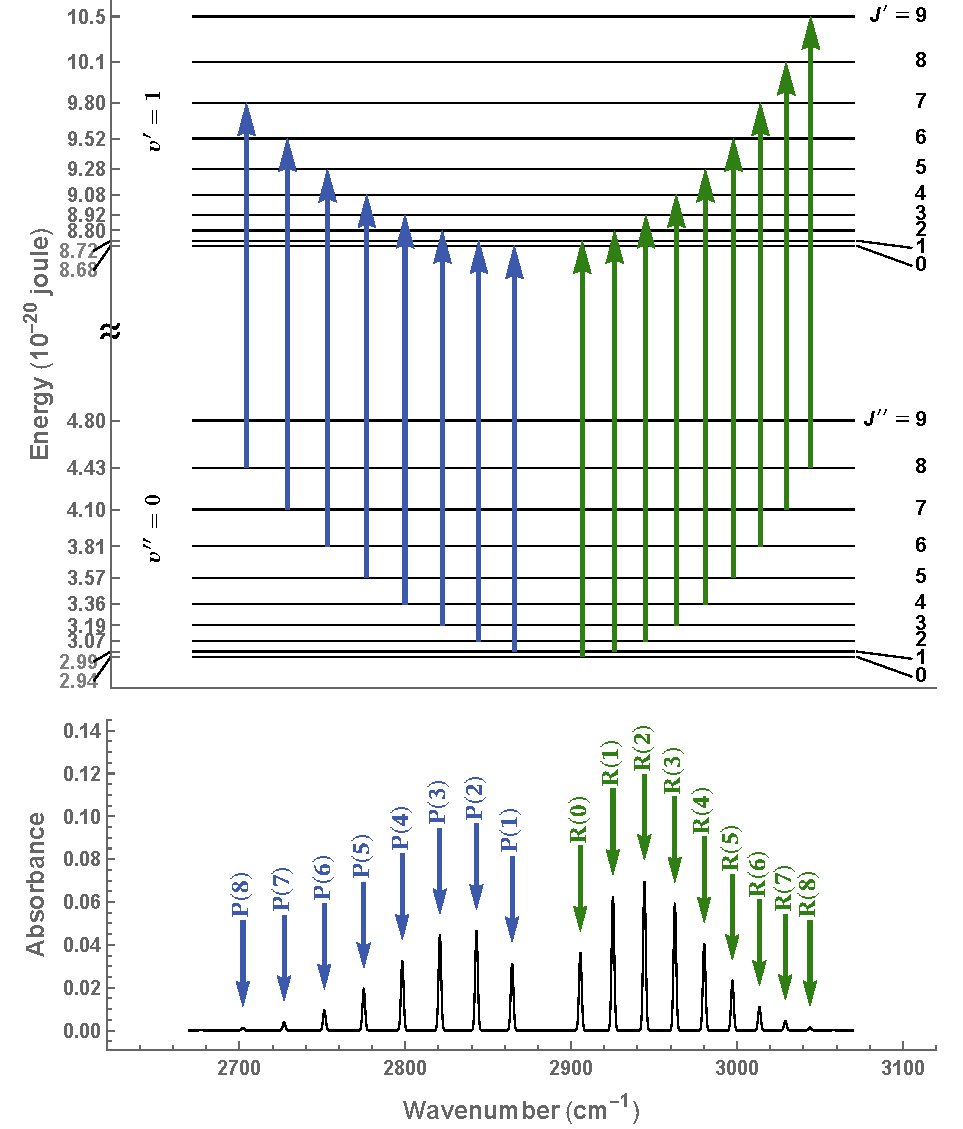
\includegraphics[width=.9\textwidth]{images/rot_energy_levels.pdf}
		\label{fig:typ_spectrum}
\end{figure}

The two series of lines given in \cref{eq:r_branch,eq:p_branch} are called \emph{R} and \emph{P} branches, respectively. 
These allowed transitions are indicated on the energy-level diagram given in \cref{fig:typ_spectrum}. 
If \( \alpha_e \) were negligible, \cref{eq:r_branch,eq:p_branch} would predict a series of equally spaced lines with separation \( 2 B_e \) except for a missing line at \( \widetilde{\nu}_0 \). 
The effect of interaction between rotation and vibration (non-zero \( \alpha_e \)) is to draw lines in the \emph{R} branch closer together and spread the lines in the \emph{P} branch farther apart, as shown for a typical spectrum in \cref{fig:typ_spectrum}. 
For convenience, let us introduce a new quantity \( m \), where \( m = J'' + 1 \) for the \emph{R} branch and \( m = -J'' \) for the \emph{P} branch, as shown in \cref{fig:typ_spectrum}. 
It is now possible to replace \cref{eq:r_branch,eq:p_branch} with a single equation:
\begin{equation}
	\widetilde{\nu}\br{m} = \widetilde{\nu}_0 + \br{2 B_e - 2 \alpha_e} m - \alpha_e m^2 \, ,
	\label{eq:both_branches1}
\end{equation}
where \( m \) takes all integral values and \( m = 0 \) yields the frequency \( \widetilde{\nu}_0 \) of the forbidden ``purely vibrational'' transition. 
If one retains the \( D_J \) term of \cref{eq:vib_rot_energies} (which assumes \( D'' = D' = D_J \)), \cref{eq:both_branches1} takes the form
\begin{equation}
	\widetilde{\nu}\br{m} = \widetilde{\nu}_0 + \br{2 B_e - 2 \alpha_e} m - \alpha_e m^2 - 4 D_J m^3 \, .
	\label{eq:both_branches2}
\end{equation}
Thus, a multiple linear regression can be performed to determine \( \widetilde{\nu}_0 \), \( B_e \), \( \alpha_e \), and \( D_J \).

% subsection selection_rules (end)

\subsection{Isotope Effect} % (fold)
\label{sub:isotope_effect}

When an isotopic substitution is made in a diatomic molecule, the equilibrium bond length, \( r_e \) and the force constant, \( k \), are unchanged, since they depend only on the behavior of the bonding electrons. 
However, the reduced mass, \( \mu \), does change, and this will affect the rotation and vibration of the molecule. 
In the case of rotation, the isotope effect can be easily stated. From the definitions of \( B_e \) and \( I \), we see that 
\begin{equation}
	\frac{B_e^*}{B_e} = \frac{\mu}{\mu^*} \, ,
	\label{eq:eff_mass_isotope_relation}
\end{equation}
where an asterisk is used to distinguish one isotopic molecule from another. 

For a harmonic oscillator model, the frequency \( \widetilde{\nu}_e \) in wavenumbers is given by 
\begin{equation}
	\widetilde{\nu}_e = \frac{1}{2 \pi c} \sqrt{\frac{k}{\mu}} \, ,
	\label{eq:ho_freq}
\end{equation}
which leads to the relation 
\begin{equation}
	\frac{\widetilde{\nu}_e^*}{\widetilde{\nu}_e} = \sqrt{\frac{\mu}{\mu^*}}\, .
	\label{eq:ho_freq_relation}
\end{equation}
The ratio \( \widetilde{\nu}_e^* / \widetilde{\nu}_e \) differs slightly from this harmonic ratio due to deviation of the true potential function from a quadratic form, as depicted in \cref{fig:potential_curves}. 
A closer approximation to the solid curve can be had by adding cubic and higher anharmonic terms to \( U\br{r} \)\sidenote{The Morse potential}, viz.,
\begin{equation}
	U\br{r} = \frac{1}{2} k \br{r - r_e}^2 + c_1 \br{r - r_e}^3 + c_2 \br{r - r_e}^4 + \ldots
	\label{eq:anharmonic_expansion}
\end{equation}
Although somewhat complicated, it can be shown\autocite{herzberg89,levine75} that the \( c_1 \) and \( c_2 \) terms yield, as the first correction to the energy levels, precisely the \( -\widetilde{\nu}_e \chi_e \br{v + {1}/{2}}^2 \) term given in \cref{eq:vib_rot_energies}. 
A similar conclusion is reached if \( U\br{r} \) is taken to have the Morse potential form given by%
\sidenote{
	The parameter \( \beta \) is determined by equating \( k_e \) to the curvature of the Morse potential at \( r = r_e \), yielding
	\begin{equation}
		\beta = \sqrt{\frac{k_e}{2 h c D_e}} \, .
		\label{eq:morse_beta}
	\end{equation}
	This three-parameter function has the desired values of \( U\br{r = r_e} = -D_e \) and \( U\br{r = \infty} = 0 \). 
	It provides a very good approximation to the real potential energy curve at all distances except \( r \ll r_e \), a region of no practical significance. 
} 
\begin{equation}
	U\br{r - r_e} = D_e \br{\br{1 - \exp{-\beta\br{r - r_e}}}^2 - 1} \, .
	\label{eq_morse_potential}
\end{equation}
In both cases, the mass dependence of \( \widetilde{\nu}_e \chi_e \) is found to be greater than for \( \widetilde{\nu}_e \) and is
\begin{equation}
	\frac{\widetilde{\nu}_e^* \chi_e^*}{\widetilde{\nu}_e \chi_e } = \frac{\mu}{\mu^*} \, .
	\label{eq:ve_isotope_relation}
\end{equation}
\Cref{eq:ho_freq_relation,eq:ve_isotope_relation} are useful in obtaining the \( \widetilde{\nu}_0^* \) counterpart of \cref{eq:forbid_transition},
\begin{equation}
	\widetilde{\nu}_0^* = \widetilde{\nu}_e^* - 2\widetilde{\nu}_e^* \chi_e^* = \widetilde{\nu}_e \sqrt{\frac{\mu}{\mu^*}} - 2 \widetilde{\nu}_e \chi_e \frac{\mu}{\mu^*} \, ,
	\label{eq:forbidden_isotope_transition} 
\end{equation}
and it is seen that a measurement of \( \widetilde{\nu}_0 \) for \ch{HCl} and \ch{DCl} suffices for a determination of \( \widetilde{\nu}_e \) and \( \widetilde{\nu}_e \chi_e \). 
Alternatively or course, the latter constants can be determined from overtone vibrations \( \br{\Delta v > 0} \) of a single isotopic form\Footcite[See Exp. 39 in][]{nibler14}. 
However, such overtones generally have low intensity and the transitions may fall outside the range of many infrared instruments, so the isotopic shift method is used in the present experiment. 

Since \ch{HCl} gas is a mixture of \ch{H^{35}Cl} and \ch{H^{37}Cl} molecules, a chlorine isotope effect will also be present. 
However, the ratio of the reduced masses is only \num{1.0015},: therefore, high resolution is required to detect this effect. 
\ch{HCl} is predominantly \ch{H^{35}Cl}, and for this experiment, we shall assume that the \ch{HCl} bands obtained are those of \ch{H^{35}Cl}. 
If deuterium is substituted for hydrogen, the ratio of the reduced masses, \( \mu\br{\ch{D^{35}Cl}} / \mu\br{\ch{H^{35}Cl}} \), is \num{1.946} and the isotope effect is quite large. 

% subsection isotope_effect (end)

\subsection[Vibrational Partition Function]{Vibrational Partition Function\autocite{levine95,mcquarrie73,lewis61}} % (fold)
\label{sub:vibrational_partition_function}

The thermodynamic quantities for an ideal gas can usually be expressed as a sum of translational, rotational, and vibrational contributions. 
We shall consider here the heat capacity at constant volume. 
At room temperature and above, the translational and rotational contributions to \( C_v \) are constants that are independent of temperature. 
For \ch{HCl} and \ch{DCl}\sidenote{diatomic, and thus linear, molecules}, the molar quantities are 
\begin{align}
	\begin{split}
		\widetilde{C}_v\br{\mtext{trans}}	&=	\frac{3}{2}R \\
		\widetilde{C}_v\br{\mtext{rot}}		&=	R \, .
	\end{split}
	\label{eq:c_v_rot_vib}
\end{align}
The vibrational contribution to \( \widetilde{C}_v \) varies with temperature and can be calculated from the vibrational partition function, \( q_\mtext{vib} \) using 
\begin{equation}
	\widetilde{C}_v\br{\mtext{vib}} = R \pdv{T}\br{T^2 \pdv{\ln{q_\mtext{vib}}{T}}} \, .
	\label{eq:vib_part_func1}
\end{equation}
The partition function, \( q_\mtext{vib} \), of \ch{HCl} or \ch{DCl} is well-approximated by the harmonic-oscillator partition function, \( q_\mtext{HO} \). 
Since the energy levels of a harmonic oscillator are given by \( \br{v + \tfrac{1}{2}} h \nu \), one obtains\autocite{levine95}
\begin{equation}
	q_\mtext{HO} = \sum_{v = 0}^\infty \exp \br{\frac{-\br{v + \tfrac{1}{2}} h \nu}{k T}} = \frac{e^{-h \nu/\br{2kT}}}{{1 - e^{-h \nu / \br{k T}}}} \, .
	\label{eq:qho_part_func}
\end{equation}
Combining \cref{eq:vib_part_func1,eq:qho_part_func}, we find 
\begin{equation}
	\widetilde{C}_v\br{\mtext{vib}} = R \frac{u^2 e^{-u/2}}{\br{1 - e^{-u}}^2} \, ,
	\label{eq:vib_part_func2}
\end{equation}
where \( u = h \nu / \br{kT} = h c \widetilde{\nu} / \br{k T} = 143.88 \widetilde{\nu} / T \). 

% subsection vibrational_partition_function (end)

% section theory (end)


\pagebreak

\section{Safety Precautions} %(fold)
\label{sec:safety}

\begin{itemize}
	\item \ch{HCl} is a strong acid should be handled cautiously. 
	\item All chemical work should be done in the fume hood and gloves should be worn at all times. 
	\item Always wear safety glasses in the laboratory.
	\item The cell used to obtain the infrared spectra is valuable and non-replaceable. 
	Handle it with extreme care. 
	The windows are made from \ch{NaCl} and are moisture sensitive. 
	Do not touch the lenses with your fingers or expose them to moisture of any kind. 
	If the cell filled with HCl breaks outside the fume hood, notify the instructor immediately and clear the area. 
\end{itemize}
% section safety (end)


\section{Procedure} % (fold)
\label{sec:procedure}

This experiment must be performed with an IR spectrometer capable of medium to high resolution (\( > \SI{2}{\wn} \) resolution). 
A high-quality grating spectrometer and most FTIR instruments are generally capable of this, and FTIR instruments don't require calibration with external gas standards. 

The infrared gas cell is constructed from a short (\SIrange{5}{10}{\cm}) length of large-diameter (\SIrange{4}{5}{\cm}) Pyrex tubing with a vacuum stopcock attached. 
Infrared-transparent windows are clamped agains O-rings at the ends of the cell or are sealed on the ends with Glyptal resin. 
For studies concentrating on the region \SIrange{4000}{500}{\wn}, \ch{NaCl} windows will suffice. 
When the spectrum of interest extends down to \SI{\sim400}{\wn}, \ch{KBr} windows are necessary. 
Both types of salt windows become ``foggy'' on prolonged exposure to a moist atmosphere and should be protected\sidenote{\emph{e.g.,} stored in a desiccator} when not in use. 
In the present experiment, inert sapphire windows with transmission down to \SI{1600}{\wn} are particularly convenient and relatively inexpensive. 

\subsection{Filling the Cell and Recording the Spectra} % (fold)
\label{sub:filling_the_cell}

Before beginning the synthesis, power on the FTIR. 
% A 50-mL two-neck round-bottom flask and a 10-cm air condenser should be washed thoroughly with soap and water followed by several rinses with distilled water.
% Then, the glassware  should be dried in an oven for approximately \SI{10}{\minute} at a temperature near \SI{110}{\celsius}.
Prior to starting, purge the 5-cm gas cell (Thermo Fisher) with nitrogen gas to clean out the cell.
This can be accomplished by attaching the tubing from the nitrogen tank regulator to one of the glass ports on the gas cell. 
Open both stopcocks on the gas cell and slowly open the needle valve on the nitrogen tank\sidenote{Ask the instructor if you are unfamiliar with the use of a regulator.} until a steady stream of gas is exiting the open port of the gas cell. 
After allowing the gas to flow for \SI{2}{\minute}, close the stopcock on the gas cell port releasing the gas and immediately close the stopcock on the port receiving the flowing gas, effectively sealing the gas cell. 
Immediately close the knob above the regulator nozzle, then close the needle valve controlling the tank's gas flow. 
Remove the tubing from the gas cell port and take the gas cell to the FTIR to obtain a background spectrum. 
Return the gas cell to the fume hood for the gas synthesis. 

% By this time, the glassware in the oven should be dry. Remove the dry glassware and place on a piece of paper towel to cool for another \SI{10}{\minute} (or until cool to the touch).
Prepare an indicator solution by dissolving \numrange{3}{4} drops of bromcresol green in \SI{300}{\mL} of DI water in a \SI{400}{\mL} beaker. 
Attach Tygon tubing to the two stems of the gas cell, lubricating with glycerin to help the tubing slide on the glass. 
Take the end of one tube and submerge it in your indicator solution.\sidenote{This will fill two roles: as a bubbler, it will prevent atmospheric gases from diffusing back into the cell; and as an indicator, it will show when sufficient \ch{HCl} has passed through the cell. \ch{HCl} is highly soluble in water, so the gaseous \ch{HCl} will quickly acidify the water.} 

To set up the rest of the apparatus, clamp a \SI{50}{\mL} round-bottom flask to a ring stand. 
Place \SI{\sim5}{\mL} of \ch{D2O} with \SI{\sim5}{\mL} concentrated \ch{HCl} in the round-bottom flask.
Prepare an air condenser (\SI{10}{\cm}) by placing a plug of glass wool at the bottom and filling the rest with \ch{CaCl2} (approximately \SI{12}{mesh}). 
Insert the stem of the condenser into a stopper, again using glycerin for lubrication, and insert the stopper into the neck of the round-bottom flask. 
Insert the end of the second tube (attached to the gas cell) into another stopper with a hole, then insert that stopper into the top of the air condenser. 
% Mix \SI{\sim5}{\mL} of \ch{D2O} with \SI{\sim5}{\mL} concentrated \ch{HCl},\sidenote{this is easiest to do in a small beaker}, then pour the mixture into the round-bottom flask via the second neck.
% Finally, insert another stopper with a hole into the second neck of the flask.
%
% With a disposable plastic pipette, obtain \SI{\sim 1}{\mL} of concentrated \ch{H2SO4}.
% Insert the pipette (\textbf{carefully} so as not to prematurely inject it) into the hole of the second stopper.
% Once you have verified that all of the holes are plugged, squeeze \numrange{1}{2} drops of sulfuric acid into the solution.
% You should see vigorous bubbling in the flask.
% At this point, open the stoppers on the gas cell.
% Continue to \emph{slowly} add sulfuric acid dropwise to the flask, watching the bubbles evolving in the indicator.

Suspend the round-bottom flask in a water bath held around \SI{80}{\celsius}. 
Gaseous \ch{HCl} will slowly evolve from the solution and bubble through the indicator solution. 
When the indicator changes color from blue to green/yellow, close the stopcocks on the gas cell and remove the round-bottom flask from the water bath. 
This procedure should take \SI{\sim20}{\min}. 
Carefully remove the tubes from the gas cell and proceed to the spectrometer for analysis. 

Make sure the experimental settings in the FTIR software are appropriate. 
The most important change to make is changing the resolution to the smallest possible value. 
This will allow you to distinguish the individual rotational transitions in the spectrum. 

An arrangement for filling the cell is shown in \cref{fig:cell_filling}.

\begin{figure}[htb]
  \centering
    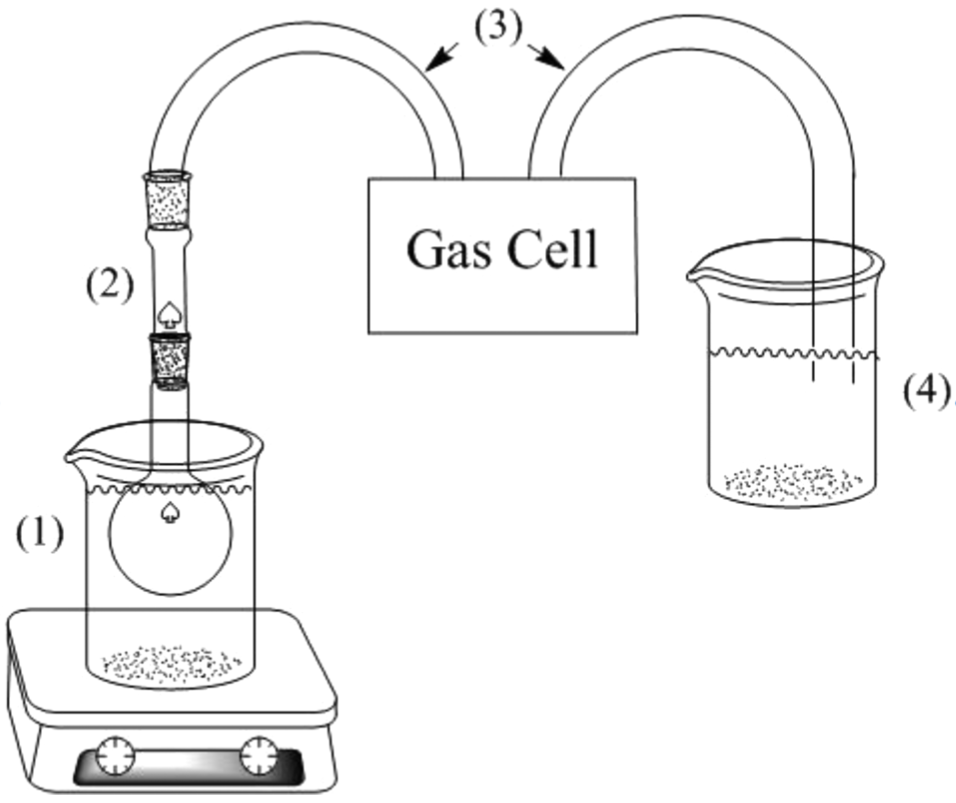
\includegraphics[width=.9\textwidth]{images/exp_setup_diagram.png}
  \caption{Experimental apparatus. (1) Water bath heating a round-bottom flask containing a mixture of \ch{HCl_{(aq)}} and \ch{DCl_{(aq)}}. (2) Condenser containing a drying agent. (3) Tygon tubing leading to and from the gas cell. (4) Beaker containing indicator solution. \\
  Figure reproduced from \cref{bigham18}.}
  \label{fig:cell_filling}
\end{figure}


% subsection filling_the_cell (end)

\subsection{Theoretical Calculations} % (fold)
\label{sub:theoretical_calculations}

The following work will be done during the second week of this lab. 
You will need to calculate the physical properties of \ch{HCl} and \ch{DCl} using Gaussian\autocite{gaussian16}, including the potential energy, equilibrium bond length, and the predicted vibrational and rotational energies for the molecule.

Using Gaussian, calculate the potential well for the \ch{HCl} molecule. 
Because of the methods used for calculation, the mass of the nuclei doesn't influence geometry, so results will be the same for the four isotopologues. 
To simplify this process, you can use the \Verb{scan} trick from from the \ch{H3O+} PES scan in the Introduction to Computational Chemistry lab.
A number of files are available for your use in the \Verb{hcl-dcl_lab} folder in JupyterLab. 
% These files should be available for you in the \Verb|PChem_Lab| folder on the desktop, but a copy is also available on Blackboard.
You will need to modify the scan parameters in the \Verb{hcl_bond.com} file (printed below).
The selected basis set and level of theory make this a quick calculation, so you can set the scan parameters quite large. 
I recommend scanning from \SIrange{0.6}{4.5}{Å} in steps less than \SI{0.05}{Å}. 
With this resolution, you should obtain a plot that gives good fidelity around the minimum while showing realistic behavior at long bond lengths. 
\gaussfileinput[title=Contents of \Verb{hcl_bond.com}]{Gaussian_simulations/hcl_bond.com}

Once you have calculated the potential energy surface for the molecule, perform an optimization and frequency analysis of the \ch{HCl} molecule.\sidenote{As outlined for \ch{H3O+} in Problem 3 in the Introduction to Computational Chemistry lab.} 
You need to do this for \ch{H^{35}Cl}, \ch{H^{37}Cl}, \ch{D^{35}Cl}, and \ch{D^{37}Cl}. 
Here is an example header for the input file for this calculation. 

\gaussfileinput[title=Template Gaussian input file vibrotational calculations on a diatomic molecule.]{Gaussian_simulations/sample.com}

Line 3 sets the theory level and basis set to reasonable values for our computational abilities and time. 
Line 4 tells Gaussian to \Verb{opt}imize the geometry, then do a \Verb{freq}uency analysis including \Verb{anharm}onic and \Verb{vib}rational-\Verb{rot}ational coupling terms. 
You will need to replace all items in angle brackets with appropriate data.
Note the addition of the \lstinline[language=Gaussian]{(Iso=<mass-num>)} option after the element labels.\sidenote{\emph{i.e.,} \lstinline[language=Gaussian]{<atom1>(Iso=<mass_num>)} should become \lstinline[language=Gaussian]{He(Iso=3)} for a \ch{^3He} atom)} 
By inserting the relevant value (total number of protons and neutrons) for your isotope (\num{2} for deuterium), you can tell Gaussian to calculate using a different atomic mass. 

You will need to import the files into your Jupyter notebook the same way you imported the files for the \ch{H3O+} molecule in the Introduction to Computational Chemistry lab. 
From there, you need to extract the values for the equilibrium bond length, \( r_0 \), and zero-point energy \( D_e \). 

You will need to search the output file for the relevant information on the energy of the ground state (relative to the zero-point energy), \( D_0 \), and the vibrational and rotational energies, \( \widetilde{\nu}_e \) and \( B_e \) (\Verb{cclib} doesn't yet parse these values).
The vibrational and rotational constants are listed in tables under the heading ``Vibrational Energies at Anharmonic Level''.
You will need to find the \emph{two} values for the first-mode vibrational energy: one calculated using a harmonic analysis, the second incorporating the effects of anharmonicity.
In this same section will be equilibrium rotational constants for the two degenerate rotational modes (labeled \Verb|Ba(y)| and \Verb|Ca(z)|) and the energy (relative to the zero-point energy) of the ground state \( (D_0) \).\sidenote{All energy values are listed in \si{\wn}.}

% subsection theoretical_calculations (end)

% section procedure (end)

\section{Data Analysis} % (fold)
\label{sec:data_analysis}

\begin{enumerate}
	\item Select your best \ch{HCl} and \ch{DCl} spectra and index the lines with the appropriate \( m \) values, as seen in \cref{fig:typ_spectrum}. 
	If the \ch{^{35}Cl}/\ch{^{37}Cl} splitting is seen, index both sets, but be sure to separate them appropriately.
	Make a table of these \( m \) values and the corresponding frequencies, \( \widetilde{\nu}\br{m} \). 
	Express the frequencies in \si{\wn} to the tenth of a \si{\wn}. 
	Then, list the differences between adjacent lines, \( \Delta{\widetilde{\nu}}\br{m} \), which will be roughly \( 2 B_e \), but will vary with \( m \). 
	\item Plot \( \Delta{\widetilde{\nu}}\br{m} \) against \( m \) and plot the trendline for the series. 
	If any values seem out of line, check the calculation for that cell. 
	\item Carry out a multiple linear least-squares fit to the data using \cref{eq:both_branches1} to determine \( \widetilde{\nu}_0 \), \( B_e \), \( \alpha_e \), and their standard errors. 
	Repeat this fitting procedure using \cref{eq:both_branches2}, noting that high \( m \) transitions will be the most important ones in determining \( D_J \), due to its \( m^3 \) dependence. 
	\item Using your values of \( \widetilde{\nu}_0 \) for \ch{HCl} and \ch{DCl}, determine \( \widetilde{\nu}_e \) and \( \widetilde{\nu}_e \chi_e \) for \ch{HCl}. From \( \widetilde{\nu}_e \), calculate \( k \) for \ch{HCl}. 
	\item Calculate \( I_e \), the moment of inertia, and \( r_e \), the internuclear distance, for both \ch{HCl} and \ch{DCl}. 
	Tabulate your results, along with your estimates  of the experimental uncertainty. Compare your results with literature values found in \textcite{kerr82}. 
	\item Using your value of \( \widetilde{\nu}_0 \) for \ch{HCl}, calculate \( \widetilde{C}_v\br{\mtext{vib}} \) at \SI{298}{\K} and at \SI{1000}{\K} from \cref{eq:vib_part_func2}. 
	Compare the spectroscopic value \( \widetilde{C}_v = 5/2 R + \widetilde{C}_v(\mtext{vib}) \) with the experimental \( \widetilde{C}_v \) value obtained from directly measured values\autocite{lewis61,spencer48} of \( \widetilde{C}_p \) and the expression \( \widetilde{C}_v = \widetilde{C}_p - R \): \( \widetilde{C}_v = \SI{20.80}{\J \per \mole\K} \) at \SI{298}{K} and \SI{23.20}{\J \per \mol\K} at \SI{1000}{\K}. 
\end{enumerate}
% section data_analysis (end)

\section{Questions and Further Thoughts} % (fold)
\label{sec:questions_and_further_thoughts}

\begin{enumerate}
	\item Compute the ratio of \( B_e^*/B_e \) and compare with the rigid-rotor prediction of \cref{eq:eff_mass_isotope_relation}. 
	How constant is \( r_e \) for \ch{HCl} and \ch{DCl}?
	\item Compute \( B_v = B_e - \alpha_e\br{v + \tfrac{1}{2}} \) for the \( v = 0 \), \num{1}, and \num{2} levels of \ch{HCl} and \ch{DCl} and, from these, obtain average \( r_v \) values for these levels. 
	Comment in your report on the changes in these distances. 
	\item Compare your \( \widetilde{\nu}_0^*/\widetilde{\nu}_0 \) ratio with the ratio \( \sqrt{\mu/\mu^*} \) expected for a harmonic oscillator. How anharmonic is the \ch{HCl} molecule: \emph{i.e.,} how large is \( \chi_e \)?
	\item Use your values of \( \widetilde{\nu}_e \) and \( \widetilde{\nu}_e \chi_e \) and \cref{eq:vib_rot_energies} to predict the frequencies of the first overtone transitions of \ch{HCl} and \ch{DCl} (ignore the rotational terms). 
	Did you observe any evidence of these overtones in your spectra? 
	\item Do your spectra show any evidence of a \ch{^{35}Cl}/\ch{^{37}Cl} isotope effect? 
	Use \cref{eq:eff_mass_isotope_relation} to calculate the splitting expected for this effect for several \emph{P} and \emph{R} branch transitions in \ch{HCl} and \ch{DCl}. 
	\item Compare your experimental results with the values deduced from your theoretical calculations. 
	For each calculation, report the values for total energy \( (D_e) \), vibration frequency \( (\widetilde{\nu}_0) \), bond length \( (r_e) \), rotation constant \( B_e \), and centrifugal distortion constant \( D_J \). 
	Additionally, you should plot the potential energy curve output by Gaussian against the theoretical Morse potential for the molecule. 
\end{enumerate}

% section questions_and_further_thoughts (end)

\section{Lab Report Guidelines} % (fold)
\label{sec:lab_report_guidelines}

As previously stated, your lab report should consist of the following parts:
\begin{description}
	\item[Title, Author and Date]
	\item[Introduction and Objective] A paragraph describing what we hope to find in this experiment, and how.
	\item[Experimental Procedure] This should be a very brief general outline of the procedure, written out as a paragraph or two. Give the make and model for any major instruments you used, as well as any important settings. For IR spectroscopy, this especially means the spectral resolution and number of scans.
	\item[Results and Discussion] This should include answers to the questions in the section ``Questions and Further Thoughts''. This should not be a separate section, but should instead be included organically in the discussion as a way of filling it out.
	\item[Conclusion]
	\item[References]
	\item[Appendix] At the very end of your report, include examples of any calculations that you did by hand. 
	Provide digital copies of the Excel (or other) files that you used to generate your graphs and copies of your Gaussian input files.
\end{description}
% section lab_report_guidelines (end)

\nocite{*}
\printbibliography[category=cited]% default title for `article` class: "References"

\DeclareFieldFormat{labelnumberwidth}{\textbullet}
\printbibliography[%
  title={Further Reading},%
  resetnumbers,%
  omitnumbers,%
	notcategory=cited,%
	]

\end{document}
